\documentclass[10pt]{article}\usepackage[]{graphicx}\usepackage[]{xcolor}
% maxwidth is the original width if it is less than linewidth
% otherwise use linewidth (to make sure the graphics do not exceed the margin)
\makeatletter
\def\maxwidth{ %
  \ifdim\Gin@nat@width>\linewidth
    \linewidth
  \else
    \Gin@nat@width
  \fi
}
\makeatother

\definecolor{fgcolor}{rgb}{0.345, 0.345, 0.345}
\newcommand{\hlnum}[1]{\textcolor[rgb]{0.686,0.059,0.569}{#1}}%
\newcommand{\hlsng}[1]{\textcolor[rgb]{0.192,0.494,0.8}{#1}}%
\newcommand{\hlcom}[1]{\textcolor[rgb]{0.678,0.584,0.686}{\textit{#1}}}%
\newcommand{\hlopt}[1]{\textcolor[rgb]{0,0,0}{#1}}%
\newcommand{\hldef}[1]{\textcolor[rgb]{0.345,0.345,0.345}{#1}}%
\newcommand{\hlkwa}[1]{\textcolor[rgb]{0.161,0.373,0.58}{\textbf{#1}}}%
\newcommand{\hlkwb}[1]{\textcolor[rgb]{0.69,0.353,0.396}{#1}}%
\newcommand{\hlkwc}[1]{\textcolor[rgb]{0.333,0.667,0.333}{#1}}%
\newcommand{\hlkwd}[1]{\textcolor[rgb]{0.737,0.353,0.396}{\textbf{#1}}}%
\let\hlipl\hlkwb

\usepackage{framed}
\makeatletter
\newenvironment{kframe}{%
 \def\at@end@of@kframe{}%
 \ifinner\ifhmode%
  \def\at@end@of@kframe{\end{minipage}}%
  \begin{minipage}{\columnwidth}%
 \fi\fi%
 \def\FrameCommand##1{\hskip\@totalleftmargin \hskip-\fboxsep
 \colorbox{shadecolor}{##1}\hskip-\fboxsep
     % There is no \\@totalrightmargin, so:
     \hskip-\linewidth \hskip-\@totalleftmargin \hskip\columnwidth}%
 \MakeFramed {\advance\hsize-\width
   \@totalleftmargin\z@ \linewidth\hsize
   \@setminipage}}%
 {\par\unskip\endMakeFramed%
 \at@end@of@kframe}
\makeatother

\definecolor{shadecolor}{rgb}{.97, .97, .97}
\definecolor{messagecolor}{rgb}{0, 0, 0}
\definecolor{warningcolor}{rgb}{1, 0, 1}
\definecolor{errorcolor}{rgb}{1, 0, 0}
\newenvironment{knitrout}{}{} % an empty environment to be redefined in TeX

\usepackage{alltt}
\usepackage[left=1in,right=1in,top=1in,bottom=1in]{geometry}
\usepackage{amsmath}
\usepackage{hyperref}
%\SweaveOpts[concordance=TRUE]
\IfFileExists{upquote.sty}{\usepackage{upquote}}{}
\begin{document}


\title{Motor vehicle colisions in NYC}
\author{Group 1 (605 - S1)}
\maketitle
\tableofcontents

\section{Introduction}
We first load the model and create new columns:
\begin{knitrout}
\definecolor{shadecolor}{rgb}{0.969, 0.969, 0.969}\color{fgcolor}\begin{kframe}
\begin{alltt}
\hlkwd{setwd}\hldef{(}\hlsng{"C:/Users/louis/Documents/Academics/Fall 2025/CMOR 605/STAT 605 Project"}\hldef{)} \hlcom{#SET TO YOUR DIRECTORY CONTAINING DATA FOLDER}
\hldef{nyc} \hlkwb{<-} \hlkwd{read.csv}\hldef{(}\hlkwc{file} \hldef{=} \hlsng{"data/Motor_Vehicle_Collisions_-_Crashes.csv"}\hldef{)}
\hldef{nyc}\hlopt{$}\hldef{CRASH.DATE} \hlkwb{<-} \hlkwd{as.Date}\hldef{(nyc}\hlopt{$}\hldef{CRASH.DATE,} \hlkwc{format} \hldef{=} \hlsng{"%m/%d/%Y"}\hldef{)}
\hldef{nyc}\hlopt{$}\hldef{BOROUGH} \hlkwb{<-} \hlkwd{factor}\hldef{(nyc}\hlopt{$}\hldef{BOROUGH)}
\hldef{nyc}\hlopt{$}\hldef{YEAR_MONTH} \hlkwb{<-} \hlkwd{format}\hldef{(nyc}\hlopt{$}\hldef{CRASH.DATE,} \hlsng{"%Y-%m"}\hldef{)}
\hldef{nyc}\hlopt{$}\hldef{YEAR} \hlkwb{<-} \hlkwd{format}\hldef{(nyc}\hlopt{$}\hldef{CRASH.DATE,} \hlsng{"%Y"}\hldef{)}
\end{alltt}
\end{kframe}
\end{knitrout}


\section{Visualizations}

\subsection{Modelling Vehicle Collisions over Time}
By grouping the collisions into each month in which they occured, we can plot a line graph showing the number of collisions over the past 13 years.
\begin{knitrout}
\definecolor{shadecolor}{rgb}{0.969, 0.969, 0.969}\color{fgcolor}\begin{kframe}
\begin{alltt}
\hldef{monthly_counts} \hlkwb{<-} \hlkwd{table}\hldef{(nyc}\hlopt{$}\hldef{YEAR_MONTH)}
\hldef{months} \hlkwb{<-} \hlkwd{names}\hldef{(monthly_counts)}
\hldef{colspermonth} \hlkwb{<-} \hlkwd{as.numeric}\hldef{(monthly_counts)}
\hldef{plot_months} \hlkwb{<-} \hlkwd{as.Date}\hldef{(}\hlkwd{paste0}\hldef{(months,} \hlsng{"-01"}\hldef{))}
\hlkwd{plot}\hldef{(plot_months, colspermonth,}
     \hlkwc{main}\hldef{=}\hlsng{"Number of Monthly Vehicle Collisions in New York City"}\hldef{,}
     \hlkwc{type}\hldef{=}\hlsng{"o"}\hldef{,}
     \hlkwc{pch}\hldef{=}\hlnum{20}\hldef{,}
     \hlkwc{xlab}\hldef{=}\hlsng{"Month"}\hldef{,}
     \hlkwc{ylab}\hldef{=}\hlsng{"Number of Collisions"}\hldef{,}
     \hlkwc{xaxt}\hldef{=}\hlsng{"n"}\hldef{,}
     \hlkwc{yaxt}\hldef{=}\hlsng{"n"}\hldef{,}
     \hlkwc{xaxs}\hldef{=}\hlsng{"i"}\hldef{,}
     \hlkwc{yaxs}\hldef{=}\hlsng{"i"}\hldef{,}
     \hlkwc{ylim}\hldef{=}\hlkwd{c}\hldef{(}\hlnum{0}\hldef{,}\hlkwd{max}\hldef{(colspermonth)}\hlopt{+}\hlnum{1000}\hldef{))}


\hldef{xticks} \hlkwb{<-} \hlkwd{seq}\hldef{(}\hlkwd{min}\hldef{(plot_months),} \hlkwd{max}\hldef{(plot_months)}\hlopt{+}\hlnum{365}\hldef{,} \hlkwc{by} \hldef{=} \hlsng{"6 months"}\hldef{)}
\hlkwd{axis.Date}\hldef{(}\hlnum{1}\hldef{,} \hlkwc{at} \hldef{= xticks,}
          \hlkwc{format} \hldef{=} \hlsng{"%b\textbackslash{}n%Y"}\hldef{,} \hlkwc{cex.axis} \hldef{=} \hlnum{0.6}\hldef{)}
\hlkwd{axis}\hldef{(}\hlnum{2}\hldef{,} \hlkwc{at} \hldef{=} \hlkwd{seq}\hldef{(}\hlnum{0}\hldef{,} \hlkwd{max}\hldef{(colspermonth)}\hlopt{+}\hlnum{1000}\hldef{,} \hlkwc{by} \hldef{=} \hlnum{1000}\hldef{),} \hlkwc{cex.axis} \hldef{=} \hlnum{0.7}\hldef{,} \hlkwc{las}\hldef{=}\hlnum{1}\hldef{)}
\hlkwd{abline}\hldef{(}\hlkwc{v} \hldef{= xticks,} \hlkwc{col} \hldef{=} \hlsng{"gray"}\hldef{,} \hlkwc{lty} \hldef{=} \hlsng{"dotted"}\hldef{)}
\end{alltt}
\end{kframe}
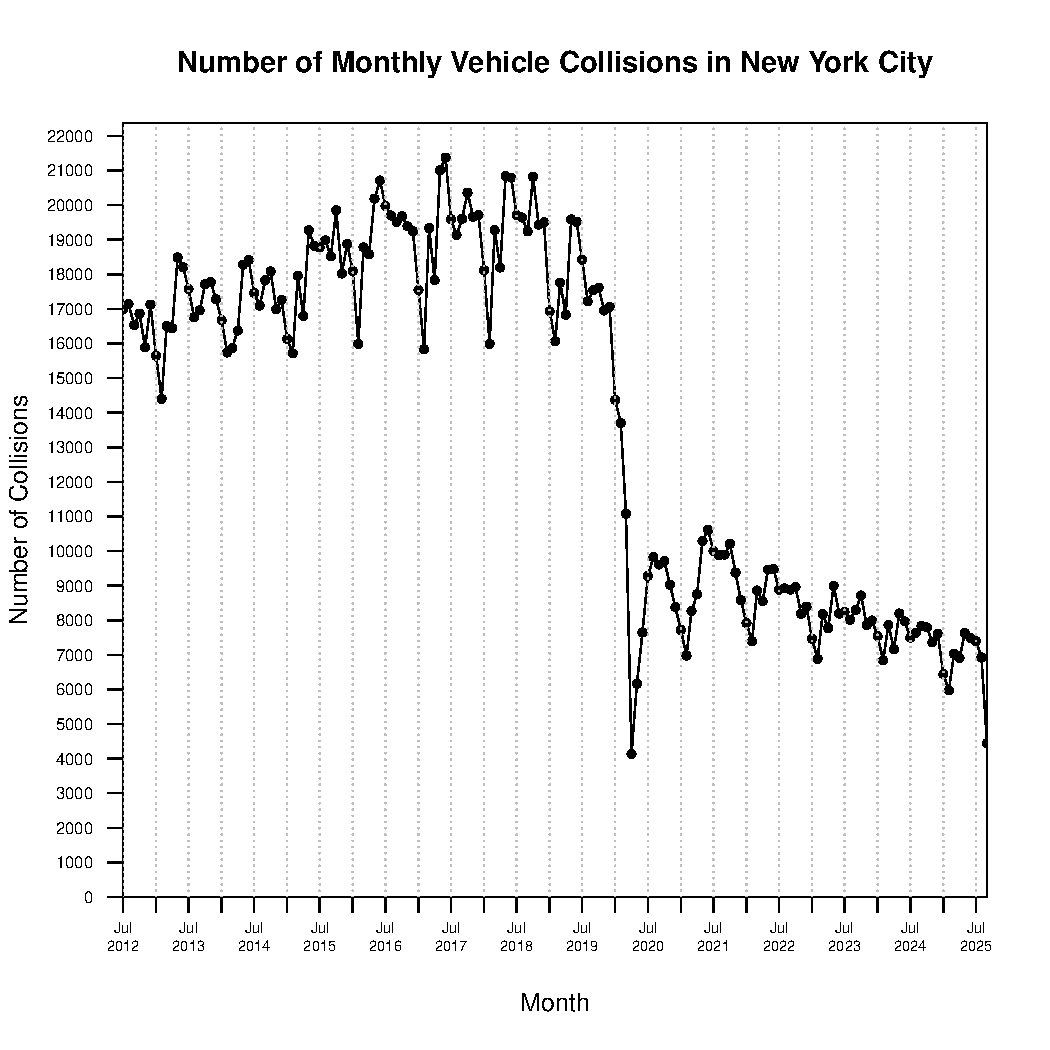
\includegraphics[width=\maxwidth]{figure/unnamed-chunk-2-1} 
\end{knitrout}
A notable trend is the sudden drop in collisions at the beginning of 2020. This is clearly due to the Covid-19 pandemic, which limited the time people spent outside their homes. What is more notable is how the number of collisions seems to even out to a much lower level than pre-pandemic. More research is needed into why we see this pattern.
\\ \\
Next, we explore the number of collisions over time within each borough. Note that a large quantity of entries from the dataset do not have a location attached, so those results are not considered for this analysis.
\begin{knitrout}
\definecolor{shadecolor}{rgb}{0.969, 0.969, 0.969}\color{fgcolor}\begin{kframe}
\begin{alltt}
\hldef{borough} \hlkwb{<-} \hlkwd{levels}\hldef{(nyc}\hlopt{$}\hldef{BOROUGH)}
\hldef{borough} \hlkwb{<-} \hldef{borough[borough} \hlopt{!=} \hlsng{""}\hldef{]}
\hldef{colors} \hlkwb{=} \hlkwd{c}\hldef{(}\hlsng{"red"}\hldef{,} \hlsng{"blue"}\hldef{,} \hlsng{"darkgreen"}\hldef{,} \hlsng{"purple"}\hldef{,} \hlsng{"orange"}\hldef{)}
\hldef{plot_months} \hlkwb{<-} \hlkwd{list}\hldef{()}
\hldef{colspermonth} \hlkwb{<-} \hlkwd{list}\hldef{()}
\hlkwa{for} \hldef{(b} \hlkwa{in} \hldef{borough)\{}
  \hldef{monthly_counts} \hlkwb{<-} \hlkwd{table}\hldef{(nyc}\hlopt{$}\hldef{YEAR_MONTH[nyc}\hlopt{$}\hldef{BOROUGH}\hlopt{==}\hldef{b])}
  \hldef{months} \hlkwb{<-} \hlkwd{names}\hldef{(monthly_counts)}
  \hldef{colspermonth[[b]]} \hlkwb{<-} \hlkwd{as.numeric}\hldef{(monthly_counts)}
  \hldef{plot_months[[b]]} \hlkwb{<-} \hlkwd{as.Date}\hldef{(}\hlkwd{paste0}\hldef{(months,} \hlsng{"-01"}\hldef{))}
\hldef{\}}

\hldef{max_col} \hlkwb{<-} \hlkwd{max}\hldef{(}\hlkwd{sapply}\hldef{(colspermonth, max))}
\hldef{min_dat} \hlkwb{<-} \hlkwd{as.Date}\hldef{(}\hlkwd{min}\hldef{(}\hlkwd{sapply}\hldef{(plot_months,min)))}
\hldef{max_dat} \hlkwb{<-} \hlkwd{as.Date}\hldef{(}\hlkwd{max}\hldef{(}\hlkwd{sapply}\hldef{(plot_months,max)))}

\hlkwd{plot}\hldef{(plot_months[[}\hlnum{1}\hldef{]], colspermonth[[}\hlnum{1}\hldef{]],}
     \hlkwc{main}\hldef{=}\hlsng{"Number of Monthly Vehicle Collisions in New York City"}\hldef{,}
     \hlkwc{type}\hldef{=}\hlsng{"l"}\hldef{,}
     \hlkwc{pch}\hldef{=}\hlnum{20}\hldef{,}
     \hlkwc{col}\hldef{= colors[}\hlnum{1}\hldef{],}
     \hlkwc{xlab}\hldef{=}\hlsng{"Month"}\hldef{,}
     \hlkwc{ylab}\hldef{=}\hlsng{"Number of Collisions"}\hldef{,}
     \hlkwc{xaxt}\hldef{=}\hlsng{"n"}\hldef{,}
     \hlkwc{yaxt}\hldef{=}\hlsng{"n"}\hldef{,}
     \hlkwc{xaxs}\hldef{=}\hlsng{"i"}\hldef{,}
     \hlkwc{yaxs}\hldef{=}\hlsng{"i"}\hldef{,}
     \hlkwc{ylim}\hldef{=}\hlkwd{c}\hldef{(}\hlnum{0}\hldef{,max_col}\hlopt{+}\hlnum{500}\hldef{))}

\hlkwa{for} \hldef{(i} \hlkwa{in} \hlnum{2}\hlopt{:}\hldef{(}\hlkwd{length}\hldef{(borough)))\{}
  \hlkwd{lines}\hldef{(plot_months[[i]], colspermonth[[i]],} \hlkwc{type}\hldef{=}\hlsng{"l"}\hldef{,} \hlkwc{pch}\hldef{=}\hlnum{20}\hldef{,} \hlkwc{col}\hldef{=colors[i])}
\hldef{\}}

\hlkwd{legend}\hldef{(}\hlsng{"topright"}\hldef{,}
       \hlkwc{legend} \hldef{= borough,}
       \hlkwc{col} \hldef{= colors,}
       \hlkwc{lty} \hldef{=} \hlnum{1}\hldef{)}


\hldef{xticks} \hlkwb{<-} \hlkwd{seq}\hldef{(min_dat, max_dat}\hlopt{+}\hlnum{365}\hldef{,} \hlkwc{by} \hldef{=} \hlsng{"6 months"}\hldef{)}
\hlkwd{axis.Date}\hldef{(}\hlnum{1}\hldef{,} \hlkwc{at} \hldef{= xticks,}
          \hlkwc{format} \hldef{=} \hlsng{"%b\textbackslash{}n%Y"}\hldef{,} \hlkwc{cex.axis} \hldef{=} \hlnum{0.6}\hldef{)}
\hlkwd{axis}\hldef{(}\hlnum{2}\hldef{,} \hlkwc{at} \hldef{=} \hlkwd{seq}\hldef{(}\hlnum{0}\hldef{, max_col}\hlopt{+}\hlnum{1000}\hldef{,} \hlkwc{by} \hldef{=} \hlnum{1000}\hldef{),} \hlkwc{cex.axis} \hldef{=} \hlnum{0.7}\hldef{,} \hlkwc{las}\hldef{=}\hlnum{1}\hldef{)}
\hlkwd{abline}\hldef{(}\hlkwc{v} \hldef{= xticks,} \hlkwc{col} \hldef{=} \hlsng{"gray"}\hldef{,} \hlkwc{lty} \hldef{=} \hlsng{"dotted"}\hldef{)}
\end{alltt}
\end{kframe}
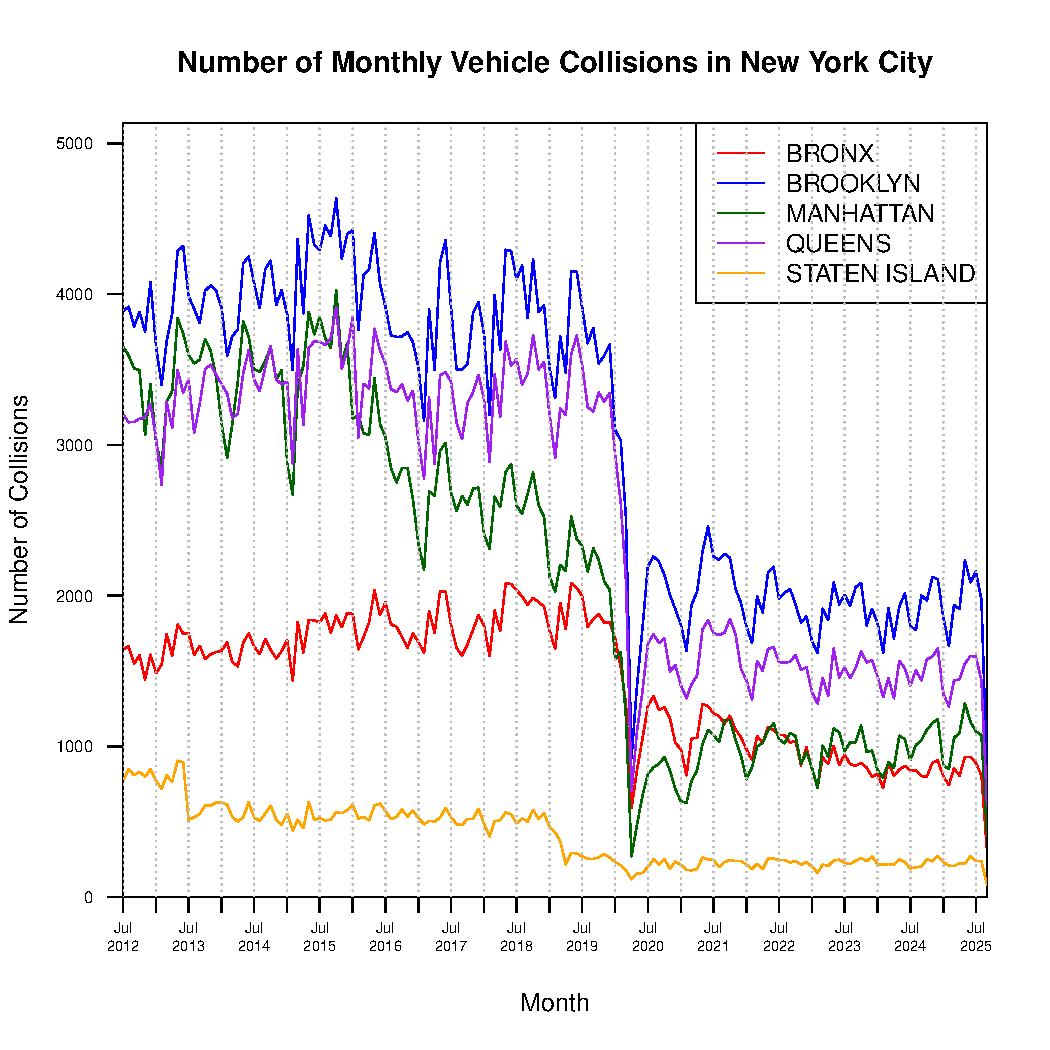
\includegraphics[width=\maxwidth]{figure/unnamed-chunk-3-1} 
\end{knitrout}
Each borough follows very similar shapes in their respective line. Further analysis to normalize by some factor, e.g. by population or road network density may provide more insight.

\subsection{Causes of Collisions}
In the dataset every entry has up to 5 `contributing factors'. Below, We see these results aggregated and the top 5 most prevalent causes displayed in a bar chart.
\begin{knitrout}
\definecolor{shadecolor}{rgb}{0.969, 0.969, 0.969}\color{fgcolor}\begin{kframe}
\begin{alltt}
\hldef{cfs} \hlkwb{<-} \hlkwd{unique}\hldef{(nyc}\hlopt{$}\hldef{CONTRIBUTING.FACTOR.VEHICLE.1)}
\hldef{cont_fact} \hlkwb{<-} \hlkwd{c}\hldef{()}
\hlkwa{for} \hldef{(f} \hlkwa{in} \hldef{cfs)\{}
  \hldef{s} \hlkwb{<-} \hlnum{0}
  \hlkwa{for} \hldef{(i} \hlkwa{in} \hlnum{1}\hlopt{:}\hlnum{5}\hldef{)\{}
    \hldef{colmn} \hlkwb{<-} \hlkwd{paste0}\hldef{(}\hlsng{"CONTRIBUTING.FACTOR.VEHICLE."}\hldef{,i)}
    \hldef{s} \hlkwb{<-} \hldef{s} \hlopt{+} \hlkwd{sum}\hldef{(nyc[[colmn]]} \hlopt{==} \hldef{f)}
  \hldef{\}}
  \hldef{cont_fact} \hlkwb{<-} \hlkwd{append}\hldef{(cont_fact,s)}
\hldef{\}}
\hlkwd{names}\hldef{(cont_fact)} \hlkwb{<-} \hldef{cfs}
\hldef{fivemost} \hlkwb{<-} \hlkwd{sort}\hldef{(cont_fact,} \hlkwc{decreasing}\hldef{=}\hlnum{TRUE}\hldef{)[}\hlnum{3}\hlopt{:}\hlnum{7}\hldef{]} \hlcom{#1st and 2nd are unspecified or null}

\hlkwd{par}\hldef{(}\hlkwc{mar} \hldef{=} \hlkwd{c}\hldef{(}\hlnum{10}\hldef{,} \hlnum{5}\hldef{,} \hlnum{4}\hldef{,} \hlnum{2}\hldef{))}
\hlkwd{barplot}\hldef{(fivemost,}
        \hlkwc{main} \hldef{=} \hlsng{"Top Contributing Factors"}\hldef{,}
        \hlkwc{col} \hldef{=} \hlkwd{c}\hldef{(}\hlsng{"darkseagreen4"}\hldef{,} \hlsng{"darkseagreen"}\hldef{,} \hlsng{"darkseagreen3"}\hldef{,} \hlsng{"darkseagreen2"}\hldef{,} \hlsng{"darkseagreen1"}\hldef{),}
        \hlkwc{las} \hldef{=} \hlnum{2}\hldef{,}
        \hlkwc{cex.names} \hldef{=} \hlnum{0.8}\hldef{,}
        \hlkwc{yaxt} \hldef{=} \hlsng{"n"}\hldef{,}
        \hlkwc{ylim} \hldef{=} \hlkwd{c}\hldef{(}\hlnum{0}\hldef{,}\hlkwd{ceiling}\hldef{(}\hlkwd{max}\hldef{(fivemost)}\hlopt{/}\hlnum{100000}\hldef{)}\hlopt{*}\hlnum{100000}\hldef{)}
        \hldef{)}

\hlkwd{title}\hldef{(}\hlkwc{ylab} \hldef{=} \hlsng{"Number of Cases"}\hldef{,} \hlkwc{line}\hldef{=}\hlnum{4}\hldef{)}

\hlkwd{axis}\hldef{(}\hlnum{2}\hldef{,} \hlkwc{at} \hldef{=} \hlkwd{seq}\hldef{(}\hlnum{0}\hldef{,} \hlkwd{ceiling}\hldef{(}\hlkwd{max}\hldef{(fivemost)}\hlopt{/}\hlnum{100000}\hldef{)}\hlopt{*}\hlnum{100000}\hldef{,} \hlkwc{by} \hldef{=} \hlnum{100000}\hldef{),}
     \hlkwc{labels} \hldef{=} \hlkwd{format}\hldef{(}\hlkwd{seq}\hldef{(}\hlnum{0}\hldef{,} \hlkwd{ceiling}\hldef{(}\hlkwd{max}\hldef{(fivemost)}\hlopt{/}\hlnum{100000}\hldef{)}\hlopt{*}\hlnum{100000}\hldef{,} \hlkwc{by} \hldef{=} \hlnum{100000}\hldef{),}
                     \hlkwc{big.mark} \hldef{=} \hlsng{","}\hldef{,}
                     \hlkwc{scientific} \hldef{=} \hlnum{FALSE}\hldef{),}
     \hlkwc{cex.axis} \hldef{=} \hlnum{0.8}\hldef{,}
     \hlkwc{las} \hldef{=} \hlnum{1}\hldef{,}
     \hldef{)}
\end{alltt}
\end{kframe}
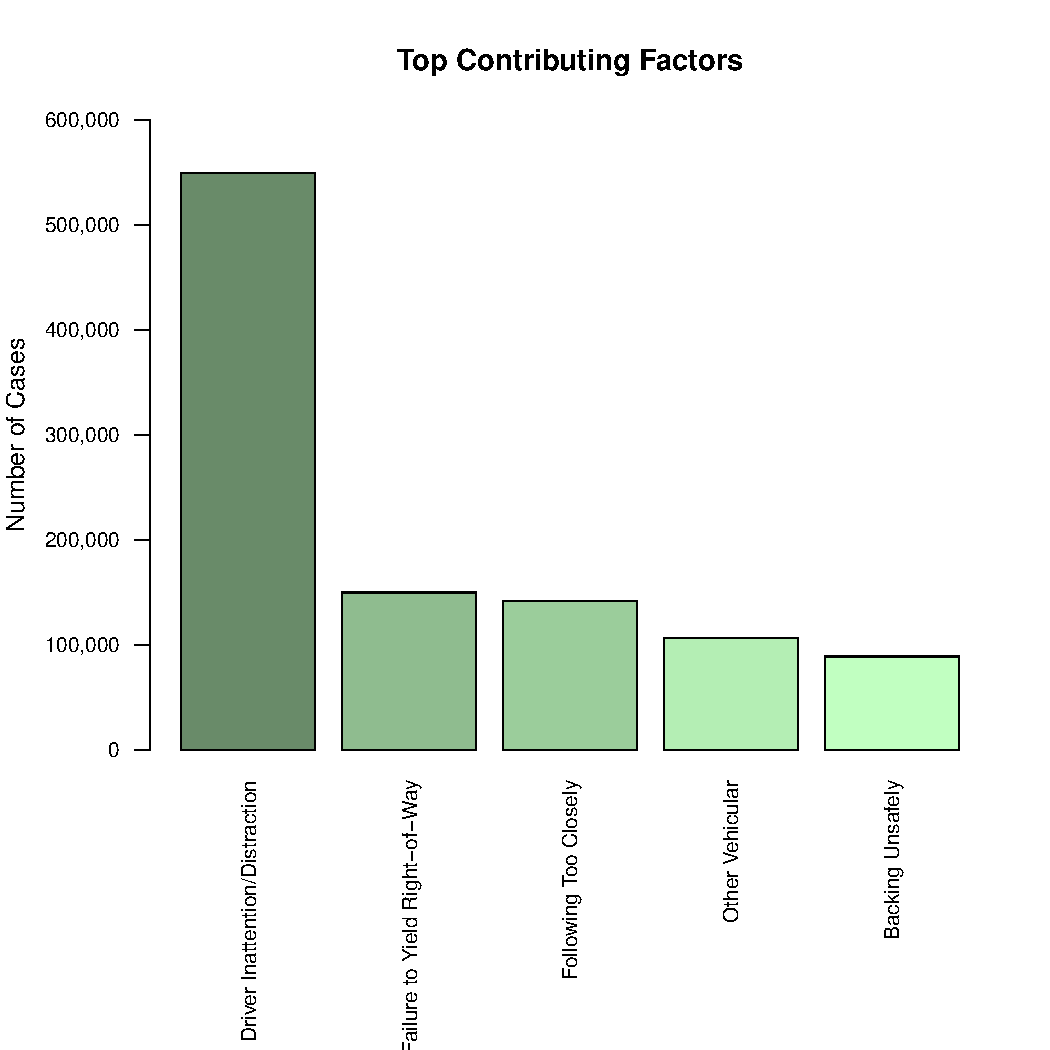
\includegraphics[width=\maxwidth]{figure/unnamed-chunk-4-1} 
\end{knitrout}
An overwhelming cause of accidents are due to driver distraction, more then 3 times the next most common.




\end{document}
